\documentclass[12pt, letterpaper]{article}
% ── Datos de la entrega ───────────────────────────────────────────────────────
\newcommand{\materia}{Desarrollo de Software Seguro}
\newcommand{\fecha}{25 de noviembre, 2026}
% ── Paquetes ──────────────────────────────────────────────────────────────────
\usepackage[spanish, es-noindentfirst, es-tabla]{babel}
\usepackage[utf8]{inputenc}
\usepackage[T1]{fontenc}
\usepackage[top=2.5cm, bottom=2.5cm, left=3cm, right=2.5cm]{geometry}
\setlength{\headheight}{14.5pt}
\usepackage{lmodern}
\usepackage{microtype}
\usepackage{setspace}
\usepackage{parskip}
\usepackage{graphicx}
\usepackage{float}
\usepackage{array}
\usepackage{booktabs}
\usepackage{tabularx}
\usepackage{longtable}
\usepackage{xcolor}
\usepackage{colortbl}
\usepackage{enumitem}
\usepackage[hidelinks]{hyperref}
\usepackage{url}
\usepackage{fancyhdr}
\usepackage{titlesec}
% Las imágenes de evidencia viven en la carpeta de seguridad del proyecto.
\graphicspath{{../seguridad/img/}{../capturas/}}
% ── Formato de secciones ──────────────────────────────────────────────────────
% Como las secciones no llevan número automático, cada título necesita su
% propio ancla (\phantomsection) para que el índice enlace al lugar correcto.
\titleformat{\section}
  {\phantomsection\normalfont\large\bfseries}{}{0em}{}[\vspace{2pt}\titlerule\vspace{2pt}]
\titleformat{\subsection}
  {\phantomsection\normalfont\normalsize\bfseries}{}{0em}{}
\titlespacing*{\section}{0pt}{16pt}{6pt}
\titlespacing*{\subsection}{0pt}{10pt}{4pt}
% Los títulos ya llevan su número escrito en el texto, así que apagamos la
% numeración automática para no duplicarla en el índice ni en el documento.
\setcounter{secnumdepth}{0}
% ── Índice ────────────────────────────────────────────────────────────────────
\usepackage{titletoc}
\titlecontents{section}[0pt]
  {\addvspace{5pt}}{\thecontentslabel\quad}{\bfseries}
  {\titlerule*[0.5pc]{.}\contentspage}
\titlecontents{subsection}[1.5em]
  {}{\thecontentslabel\quad}{}
  {\titlerule*[0.5pc]{.}\contentspage}
% ── Encabezado y pie de página ────────────────────────────────────────────────
\pagestyle{fancy}
\fancyhf{}
\renewcommand{\headrulewidth}{0.4pt}
\fancyhead[L]{\small\textit{\materia}}
\fancyhead[R]{\small\textit{Reyna, B.J.}}
\fancyfoot[C]{\small\thepage}
% ── Espaciado ─────────────────────────────────────────────────────────────────
\setlength{\parindent}{0pt}
\setlength{\parskip}{7pt}
\onehalfspacing
\setlist{itemsep=2pt, topsep=2pt, parsep=0pt, leftmargin=*}
\setlength{\LTpre}{6pt}
\setlength{\LTpost}{6pt}
\urlstyle{same}
\newcolumntype{L}[1]{>{\raggedright\arraybackslash}p{#1\linewidth}}
% ─────────────────────────────────────────────────────────────────────────────
\begin{document}
% ═══════════════════════════ PORTADA ═════════════════════════════════════════
\pagenumbering{roman}
\thispagestyle{empty}
\begin{center}
  \vspace*{1.2cm}
  {\large \textbf{Universidad Autónoma de Nuevo León}}\\[0.2cm]
  {\normalsize Facultad de Ciencias Físico Matemáticas}\\[1cm]
  {\large \textsc{\materia}}\\[0.4cm]
  {\normalsize \textit{Proyecto Integrador Académico, Semanas 3, 4 y 5}}\\[2.4cm]
  {\LARGE \textbf{Sistema QR de mantenimiento de equipos}}\\[0.5cm]
  {\Large \textbf{Implementación, verificación y aseguramiento}}\\[1.2cm]
  {\large \textit{Entregable 2}}\\[2cm]
  \renewcommand{\arraystretch}{1.6}
  \begin{tabular}{r l}
    \textbf{Integrantes:} & Cesar Oziel Guajardo Rodríguez, 2053865 \\
                          & Brandon Jahir Reyna Marroquín, 1950966 \\
                          & Johan Joel Rodríguez Medina, 2055393 \\
                          & Diego Ángel Torres Azua, 2069158 \\
    \textbf{Materia:}     & \materia \\
    \textbf{Maestro:}     & Luis Ángel Gutiérrez Rodríguez \\
    \textbf{Fecha:}       & \fecha \\
  \end{tabular}
\end{center}
\newpage
% ═══════════════════════════ ÍNDICE ══════════════════════════════════════════
\renewcommand{\contentsname}{Índice}
{\singlespacing\setlength{\parskip}{0pt}%
\tableofcontents}
\newpage
\pagenumbering{arabic}
% ═══════════════════════════ CONTENIDO ═══════════════════════════════════════

\section{1. Introducción}

En este documento presentamos el segundo entregable del Proyecto Integrador Académico, que corresponde a las semanas 3, 4 y 5. En el primer entregable definimos el sistema, sus requisitos de seguridad y su modelo de amenazas. En esta etapa implementamos ese diseño y, sobre todo, lo pusimos a prueba: lo revisamos con herramientas de análisis, lo atacamos dentro de un entorno controlado, corregimos lo que encontramos y volvimos a probar para comprobar que las correcciones funcionan.

Seguimos la misma lógica del primer entregable, que relaciona cada amenaza con su riesgo, su mitigación, su implementación, su prueba y su resultado. La diferencia es que ahora las columnas de prueba y de resultado se llenan con evidencia real, que acompañamos con capturas de cada herramienta y de cada prueba. Todas las pruebas se hicieron sobre una copia local del sistema con datos ficticios, nunca contra sistemas de terceros.

El código fuente del proyecto está en \url{https://github.com/betaup/qr-mantenimiento}.

% ─────────────────────────────────────────────────────────────────────────────
\section{2. Implementación segura}

\textit{Sección en desarrollo. Describirá cómo se implementaron la autenticación, la autorización, la validación de entradas y la protección de la información sensible.}

% ─────────────────────────────────────────────────────────────────────────────
\section{3. Análisis estático y de dependencias}

El análisis estático revisa el código sin ejecutarlo, en busca de patrones que suelen causar vulnerabilidades. Lo complementamos con una revisión de las dependencias, ya que buena parte del código que corre en el sistema no lo escribimos nosotros sino que viene de librerías externas. Ejecutamos ambos análisis el 25 de noviembre de 2026, antes de hacer cualquier corrección, para tener un punto de partida.

\subsection{Herramientas}

\begingroup\small\setlength{\tabcolsep}{4pt}\renewcommand{\arraystretch}{1.25}
\begin{longtable}{L{0.30}L{0.18}L{0.45}}
\toprule
\textbf{Herramienta} & \textbf{Versión} & \textbf{Qué revisa} \\
\midrule
\endfirsthead
\toprule
\textbf{Herramienta} & \textbf{Versión} & \textbf{Qué revisa} \\
\midrule
\endhead
\bottomrule
\endfoot
ESLint con eslint-plugin-security & 9.39.5 y 3 & Patrones peligrosos como \texttt{eval}, expresiones regulares vulnerables y accesos dinámicos a objetos y archivos. \\
Reglas de Next.js y TypeScript & 16.4.6 & Errores comunes de React, Next.js y tipos. \\
Compilador de TypeScript & 5.9 & Errores de tipos en todo el proyecto, en modo estricto. \\
npm audit & 11.19.0 & Vulnerabilidades conocidas en las dependencias, según la base de avisos de GitHub. \\
Revisión manual & & Lógica de autorización, manejo de sesiones y uso de cabeceras de la petición. \\
\end{longtable}
\endgroup

\subsection{Análisis del código}

ESLint encontró seis avisos y ningún error, todos de la regla \texttt{detect-object-injection} (figura \ref{fig:eslint-inicial}). Esta regla avisa cada vez que se lee un objeto usando una clave variable, porque si esa clave la controlara un atacante podría leer propiedades internas como \texttt{\_\_proto\_\_}.

\begin{figure}[H]
  \centering
  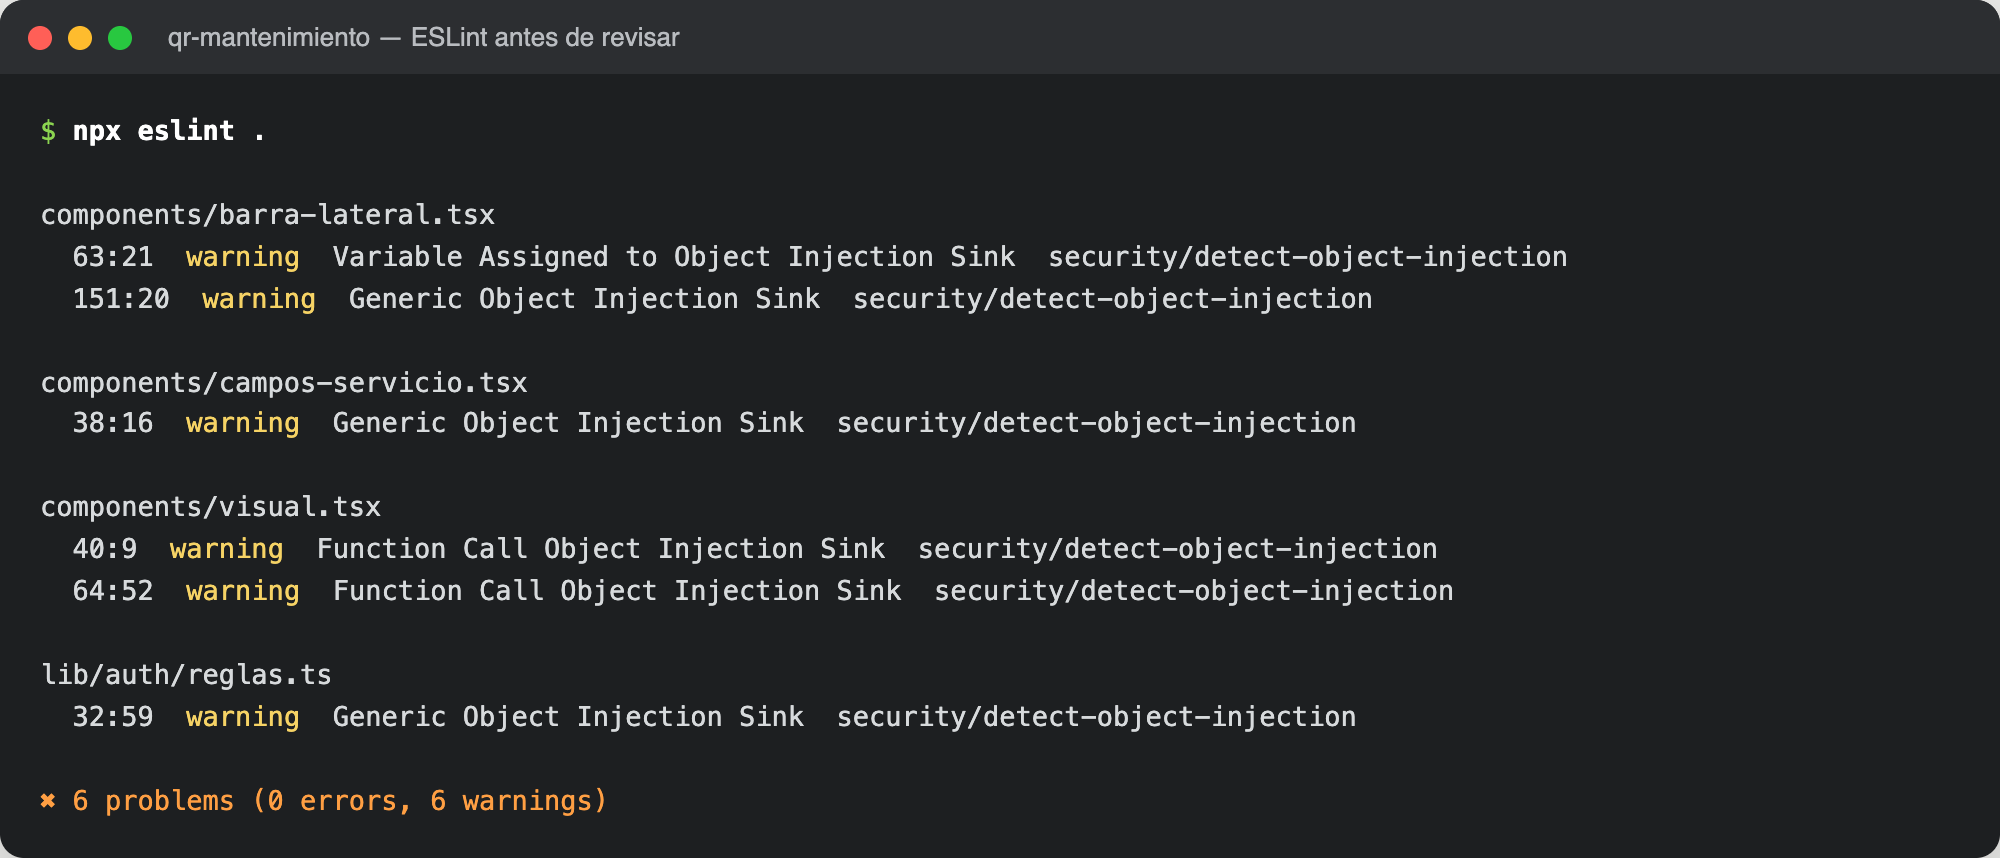
\includegraphics[width=\linewidth]{p1-eslint-inicial.png}
  \caption{Resultado inicial de ESLint con las reglas de seguridad.}
  \label{fig:eslint-inicial}
\end{figure}

Revisamos los seis casos uno por uno y concluimos que son falsos positivos. En todos la clave tiene un tipo cerrado, como el rol del usuario o el tipo de servicio, y nunca viene directamente de una petición: el rol sale de la sesión y los tipos se validan antes con Zod. Para no ignorar la regla por completo, marcamos cada caso en el código con un comentario que explica la razón. Así el análisis queda limpio y cualquier aviso nuevo se nota de inmediato (figura \ref{fig:eslint-final}).

\begingroup\small\setlength{\tabcolsep}{4pt}\renewcommand{\arraystretch}{1.25}
\begin{longtable}{L{0.36}L{0.08}L{0.25}L{0.24}}
\toprule
\textbf{Archivo} & \textbf{Línea} & \textbf{Código} & \textbf{Clasificación} \\
\midrule
\endfirsthead
\toprule
\textbf{Archivo} & \textbf{Línea} & \textbf{Código} & \textbf{Clasificación} \\
\midrule
\endhead
\bottomrule
\endfoot
\nolinkurl{components/barra-lateral.tsx} & 63 & \texttt{SECCIONES[rol]} & Falso positivo \\
\nolinkurl{components/barra-lateral.tsx} & 151 & \texttt{NOMBRE\_DE\_ROL[rol]} & Falso positivo \\
\nolinkurl{components/campos-servicio.tsx} & 38 & \texttt{NOMBRE\_DE\_TIPO[valor]} & Falso positivo \\
\nolinkurl{components/visual.tsx} & 40 & \texttt{TONOS[tono]} & Falso positivo \\
\nolinkurl{components/visual.tsx} & 64 & \texttt{PUNTOS[tono]} & Falso positivo \\
\nolinkurl{lib/auth/reglas.ts} & 32 & \texttt{PLAZOS[rol]} & Falso positivo \\
\end{longtable}
\endgroup

\begin{figure}[H]
  \centering
  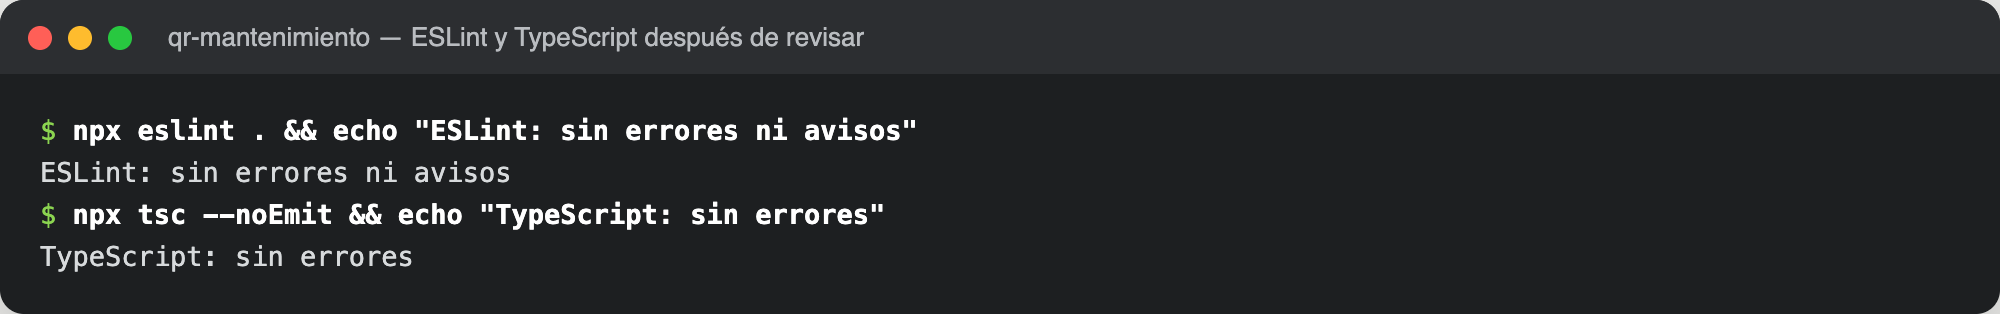
\includegraphics[width=\linewidth]{p1-eslint-final.png}
  \caption{ESLint y TypeScript sin errores ni avisos después de revisar los falsos positivos.}
  \label{fig:eslint-final}
\end{figure}

\subsection{Revisión de dependencias}

La revisión de dependencias fue más reveladora. npm audit reportó 17 paquetes vulnerables, de los cuales 2 son críticos, 4 altos y 11 moderados (figura \ref{fig:audit}). Al quedarnos solo con las dependencias de producción el número baja a 8, con 4 altos y 4 moderados (figura \ref{fig:audit-prod}).

\begin{figure}[H]
  \centering
  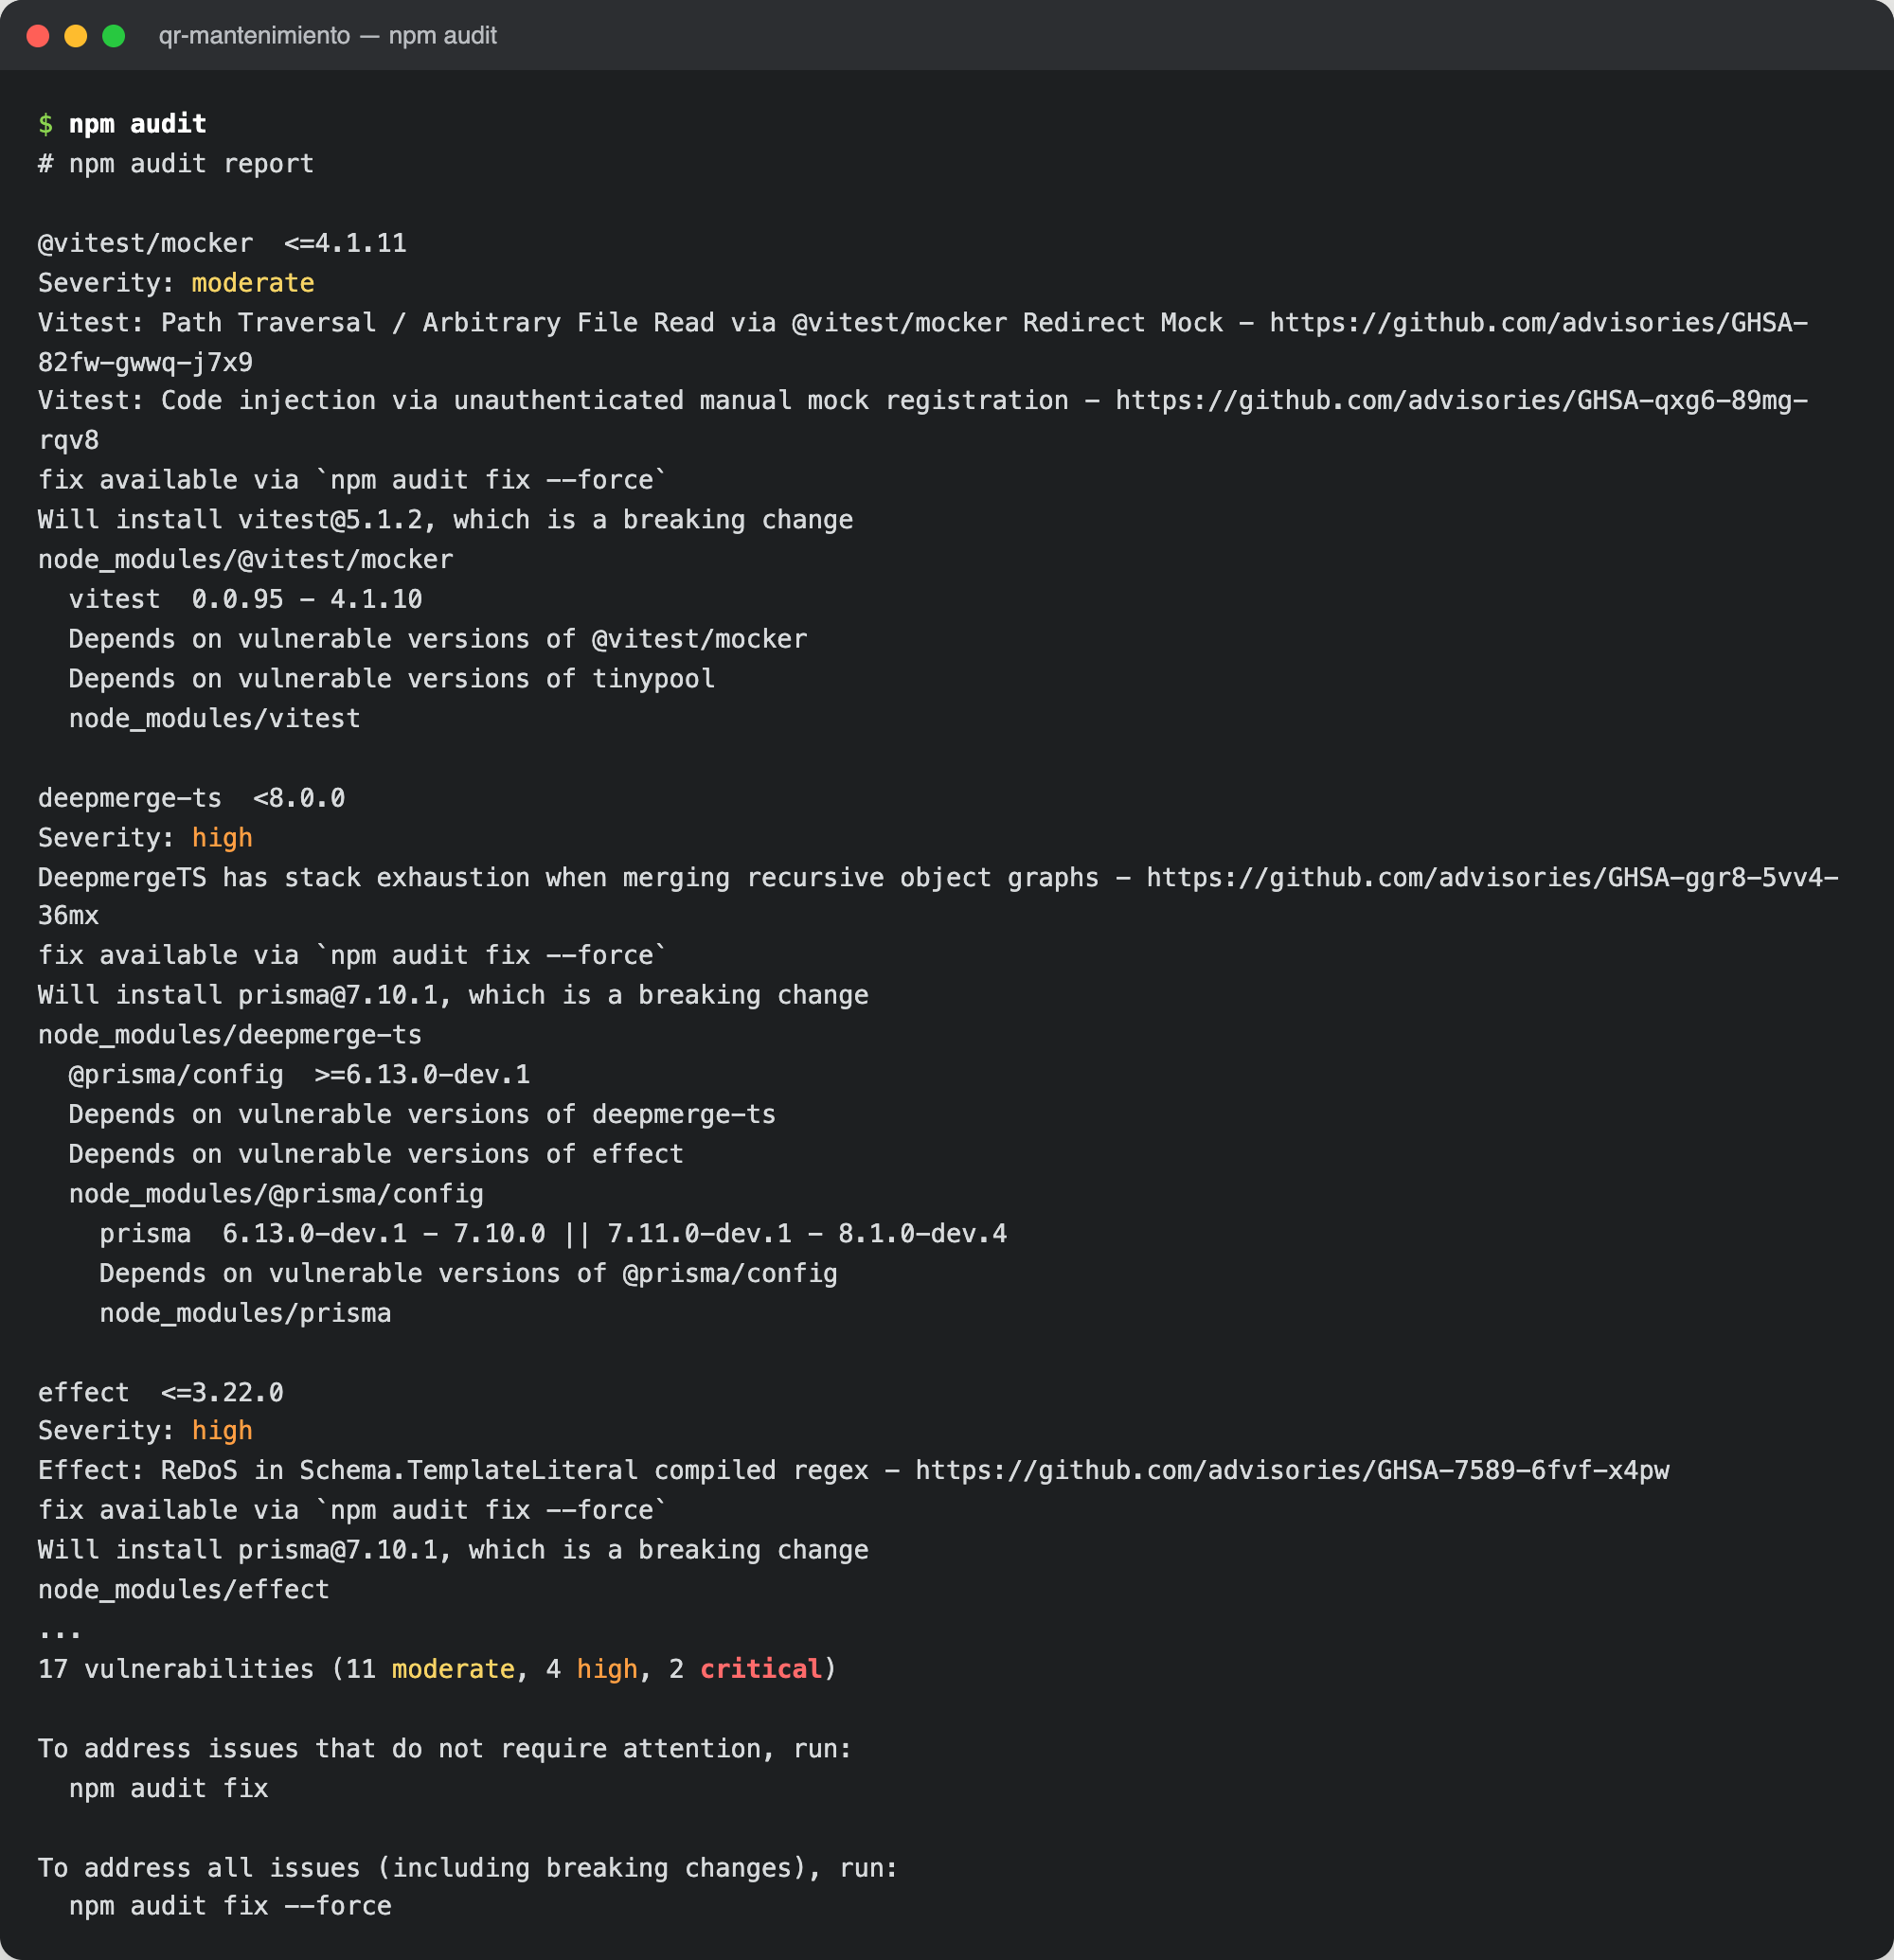
\includegraphics[width=\linewidth]{p1-npm-audit.png}
  \caption{Inicio y resumen del reporte de npm audit sobre todas las dependencias.}
  \label{fig:audit}
\end{figure}

\begin{figure}[H]
  \centering
  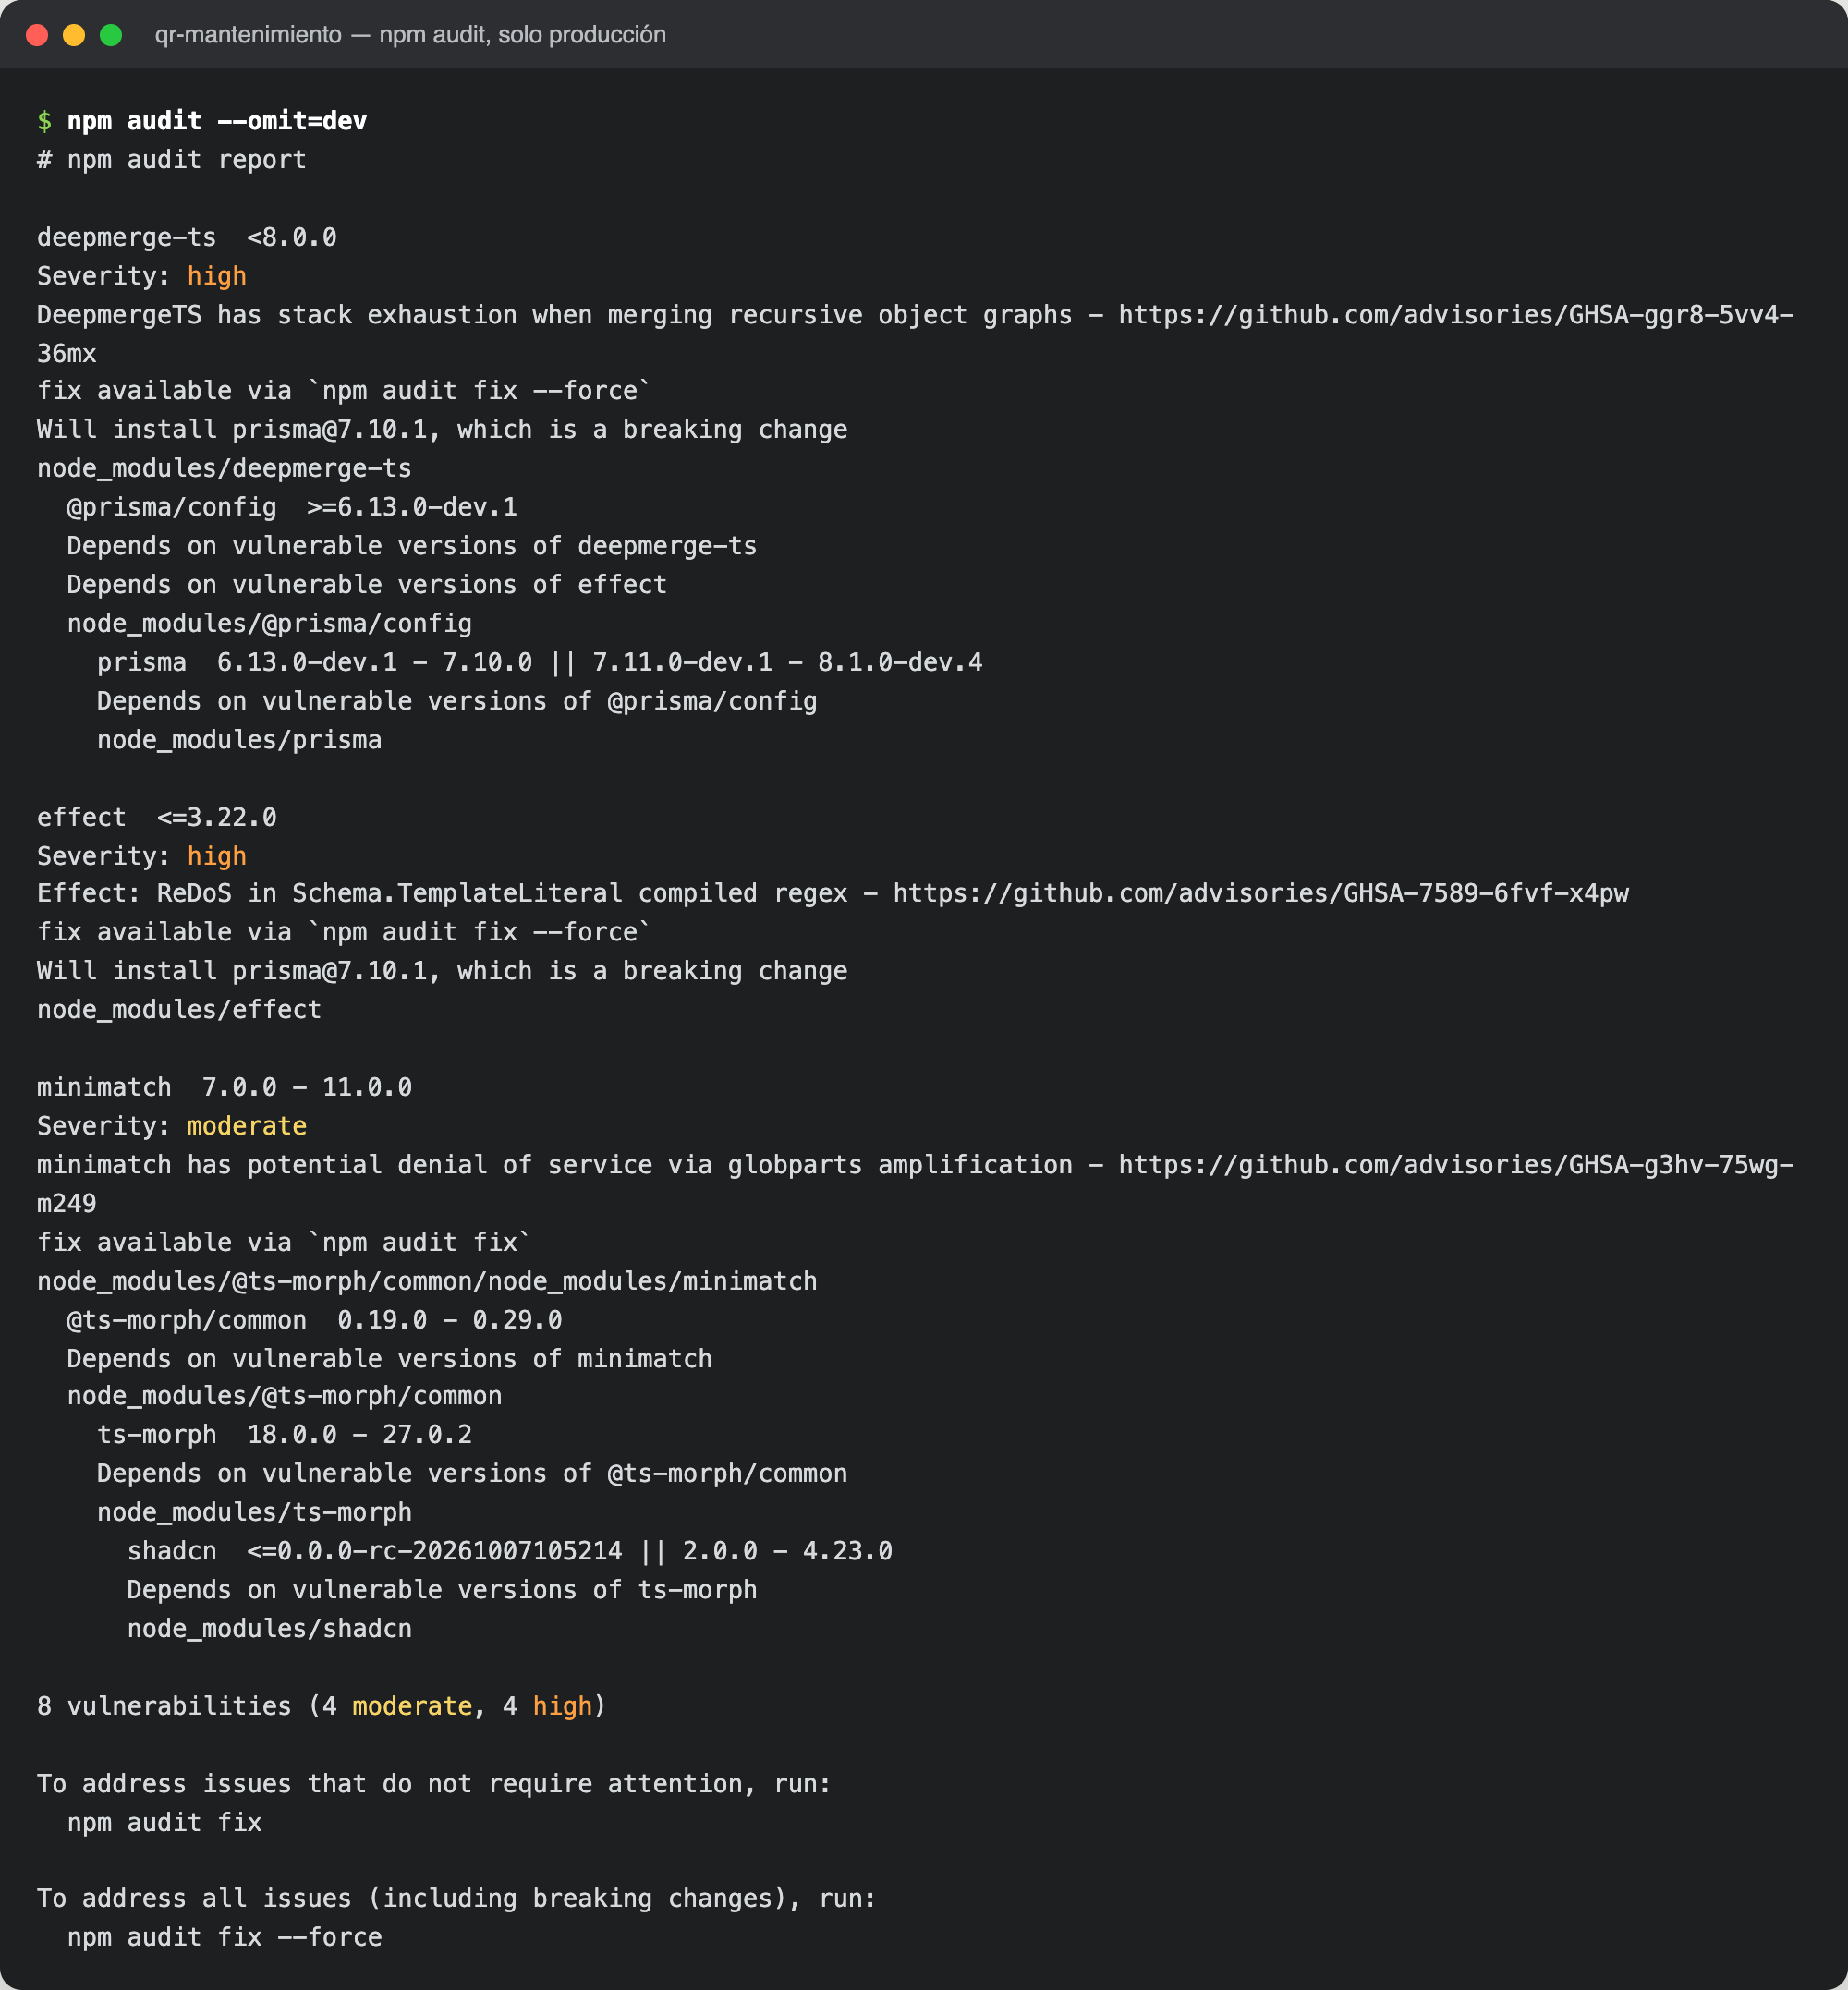
\includegraphics[width=\linewidth]{p1-npm-audit-produccion.png}
  \caption{Reporte de npm audit solo sobre las dependencias de producción.}
  \label{fig:audit-prod}
\end{figure}

\begingroup\small\setlength{\tabcolsep}{4pt}\renewcommand{\arraystretch}{1.25}
\begin{longtable}{L{0.17}L{0.11}L{0.11}L{0.24}L{0.13}L{0.14}}
\toprule
\textbf{Paquete} & \textbf{Versión} & \textbf{Severidad} & \textbf{Aviso} & \textbf{Llega por} & \textbf{Alcance} \\
\midrule
\endfirsthead
\toprule
\textbf{Paquete} & \textbf{Versión} & \textbf{Severidad} & \textbf{Aviso} & \textbf{Llega por} & \textbf{Alcance} \\
\midrule
\endhead
\bottomrule
\endfoot
tinypool & 1.1.1 & Crítica & GHSA-5gmw-xhrv-c9v3, GHSA-85c8-ppgw-ccpr & vitest & Desarrollo \\
vitest y @vitest/mocker & 3.2.7 & Moderada & GHSA-82fw-gwwq-j7x9, GHSA-qxg6-89mg-rqv8 & Directa & Desarrollo \\
deepmerge-ts & 7.1.5 & Alta & GHSA-ggr8-5vv4-36mx & prisma & Producción \\
effect & 3.21.0 & Alta & GHSA-7589-6fvf-x4pw & prisma & Producción \\
prisma y @prisma/config & 6.19.3 & Alta & Por las dos anteriores & Directa & Producción \\
minimatch & 7 a 11.0.0 & Moderada & GHSA-g3hv-75wg-m249 & shadcn y typescript-eslint & Ambos \\
shadcn y ts-morph & 4.23.0 & Moderada & Por minimatch & Directa & Producción \\
typescript-eslint & 8 & Moderada & Por minimatch & eslint-config-next & Desarrollo \\
\end{longtable}
\endgroup

Al analizar de dónde venía cada vulnerabilidad notamos tres cosas. Primero, las dos críticas están en \texttt{tinypool}, que solo usa el ejecutor de pruebas, así que no llegan a la aplicación en producción, aunque sí afectan al equipo de quien corre las pruebas y al servidor de integración continua. Segundo, \texttt{prisma} aparece en producción porque el cliente de Prisma lo pide como dependencia, pero las vulnerabilidades altas están en la configuración de su herramienta de línea de comandos y no en el cliente que corre dentro de la aplicación. Tercero, \texttt{shadcn} es una herramienta que solo usamos para agregar componentes y que, por error, quedó instalada como dependencia de producción.

\subsection{Hallazgos de la revisión manual}

Además de las herramientas, revisamos a mano las partes más sensibles del código, en especial la autorización, las sesiones y el uso de datos que llegan en la petición. Encontramos dos problemas que ninguna herramienta había señalado.

El primero, H-01, está en la función que obtiene la dirección IP del cliente (figura \ref{fig:h01}). La toma de la cabecera \texttt{X-Forwarded-For} sin comprobar que la haya puesto un proxy de confianza. Como cualquier cliente puede enviar esa cabecera con el valor que quiera, un atacante podría cambiar su IP en cada intento para esquivar el límite de intentos por dirección IP, y además dejaría direcciones falsas en la bitácora.

\begin{figure}[H]
  \centering
  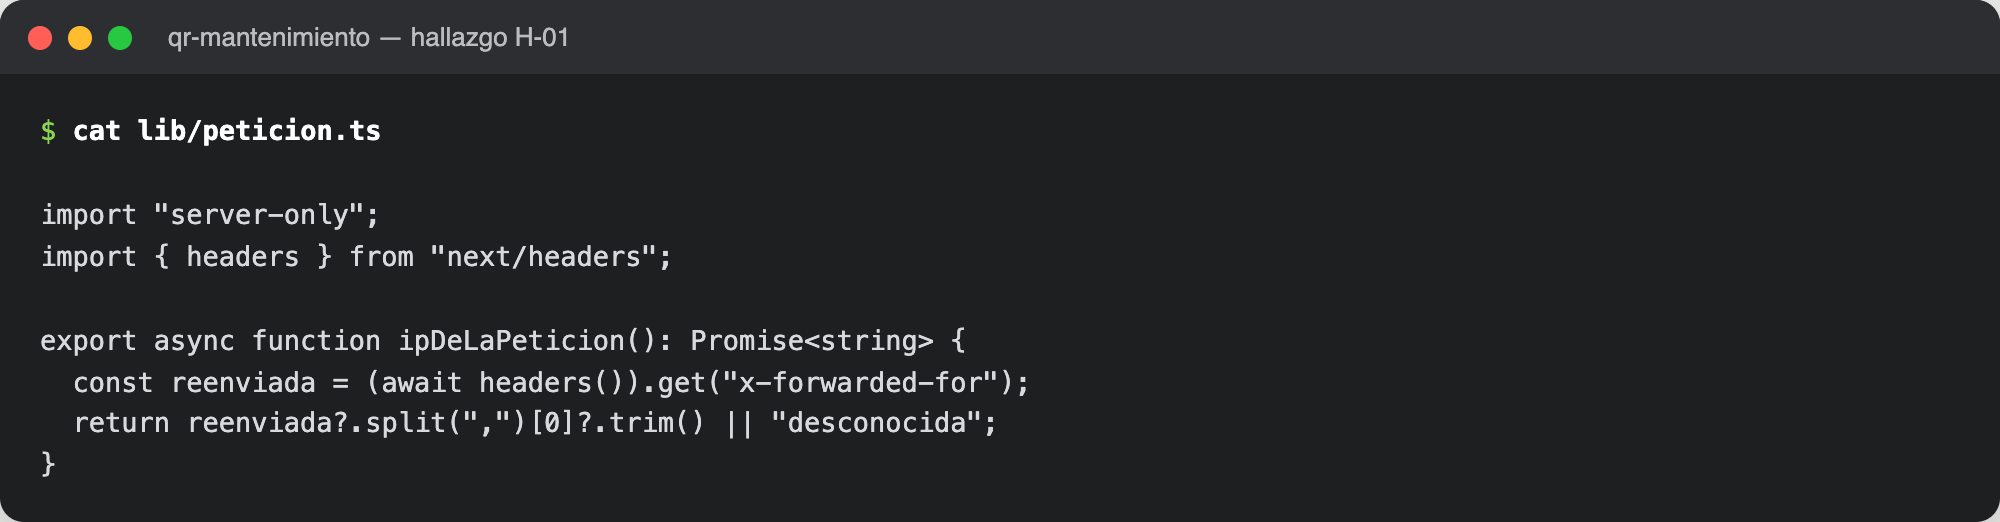
\includegraphics[width=\linewidth]{p1-h01-ip.png}
  \caption{H-01. La IP se toma de una cabecera que controla el cliente.}
  \label{fig:h01}
\end{figure}

El segundo, H-02, está en la función que quita una asignación (figura \ref{fig:h02}). La pantalla solo permite quitar asignaciones de hoy en adelante, pero la función del servidor no revisa la fecha. Una petición hecha a mano podría borrar asignaciones de días pasados y alterar el registro de quién atendió cada equipo.

\begin{figure}[H]
  \centering
  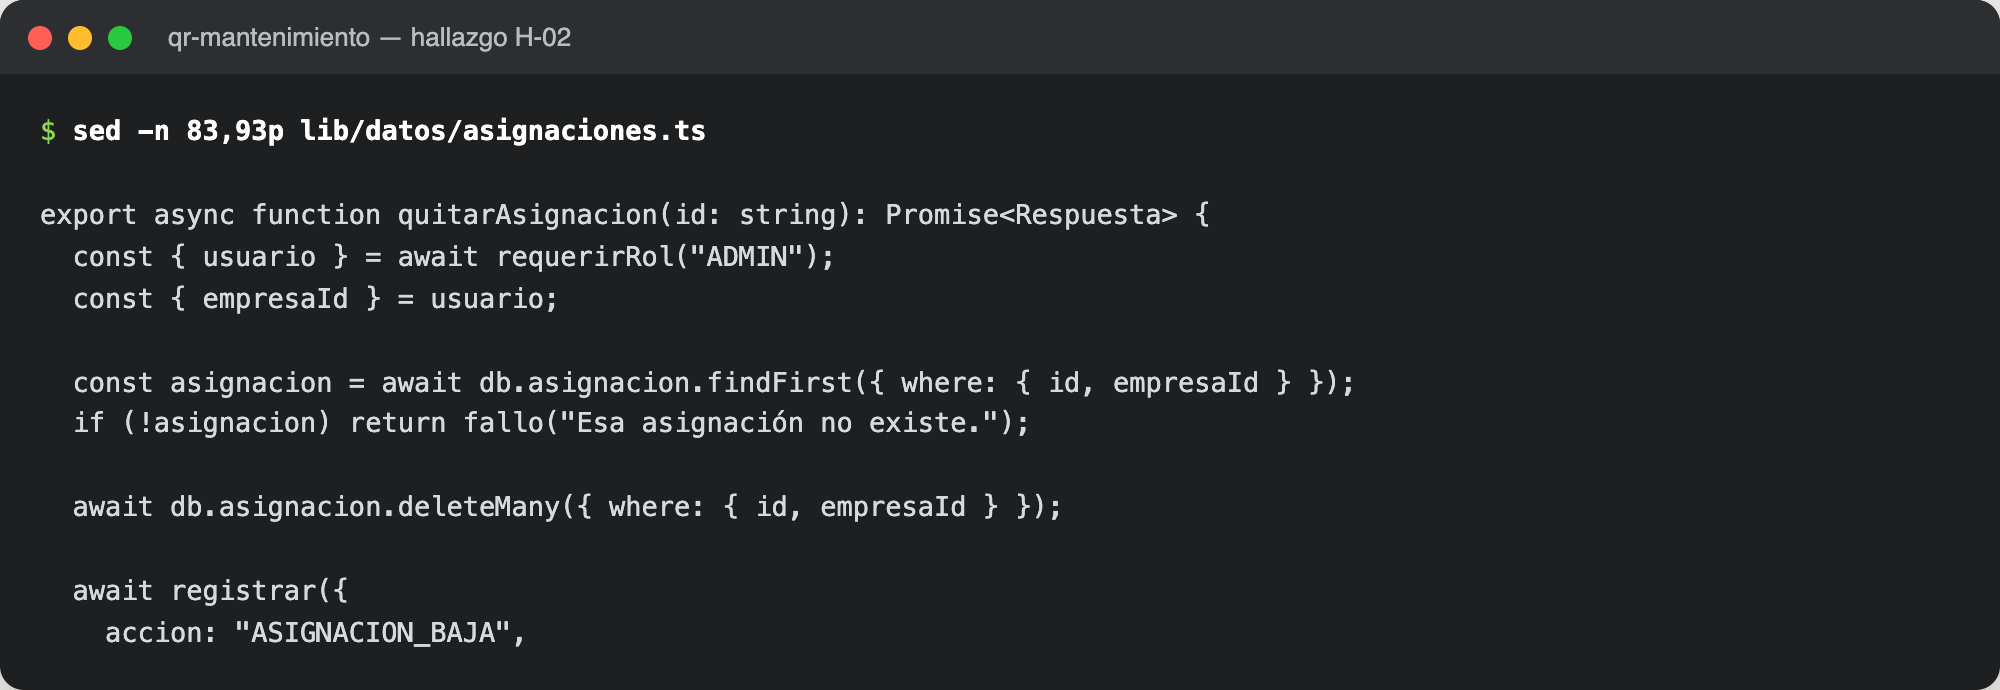
\includegraphics[width=\linewidth]{p1-h02-asignaciones.png}
  \caption{H-02. La función que quita asignaciones no revisa la fecha.}
  \label{fig:h02}
\end{figure}

\begingroup\small\setlength{\tabcolsep}{4pt}\renewcommand{\arraystretch}{1.25}
\begin{longtable}{L{0.08}L{0.52}L{0.20}L{0.13}}
\toprule
\textbf{ID} & \textbf{Hallazgo} & \textbf{Origen} & \textbf{Severidad} \\
\midrule
\endfirsthead
\toprule
\textbf{ID} & \textbf{Hallazgo} & \textbf{Origen} & \textbf{Severidad} \\
\midrule
\endhead
\bottomrule
\endfoot
H-01 & La IP del cliente se toma de una cabecera que el cliente puede falsificar. & Revisión manual & Media \\
H-02 & Se pueden quitar asignaciones de días pasados con una petición hecha a mano. & Revisión manual & Baja \\
H-03 & Una herramienta de desarrollo, shadcn, está instalada como dependencia de producción. & npm audit & Baja \\
H-04 & Hay 17 dependencias con vulnerabilidades conocidas, dos de ellas críticas. & npm audit & Alta \\
\end{longtable}
\endgroup

Estos cuatro hallazgos pasan al registro de vulnerabilidades de la sección 5, donde se clasifican con detalle. Antes de corregirlos los confirmamos con pruebas dinámicas, que se describen en la sección 4.

% ─────────────────────────────────────────────────────────────────────────────
\section{4. Pruebas dinámicas de seguridad}

\textit{Sección en desarrollo.}

\section{5. Registro y clasificación de vulnerabilidades}

\textit{Sección en desarrollo.}

\section{6. Corrección y revalidación}

\textit{Sección en desarrollo.}

\section{7. Verificación de requisitos y mitigación de amenazas}

\textit{Sección en desarrollo.}

\section{8. Integración continua y automatización}

\textit{Sección en desarrollo.}

\section{9. Dependencias y mecanismos criptográficos}

\textit{Sección en desarrollo.}

\section{10. Conclusiones}

\textit{Sección en desarrollo.}

% ═══════════════════════════ REFERENCIAS ═════════════════════════════════════
\newpage
\begin{thebibliography}{9}
\setlength{\itemsep}{5pt}

\bibitem{eslintsec} eslint-community. (s.f.). \textit{eslint-plugin-security}. GitHub. \url{https://github.com/eslint-community/eslint-plugin-security}

\bibitem{npmaudit} npm. (s.f.). \textit{npm-audit}. npm Docs. \url{https://docs.npmjs.com/cli/commands/npm-audit}

\bibitem{ghsa} GitHub. (s.f.). \textit{GitHub Advisory Database}. \url{https://github.com/advisories}

\bibitem{xff} Mozilla. (s.f.). \textit{X-Forwarded-For}. MDN Web Docs. \url{https://developer.mozilla.org/en-US/docs/Web/HTTP/Headers/X-Forwarded-For}

\bibitem{asvs} OWASP Foundation. (2021). \textit{OWASP Application Security Verification Standard}. \url{https://owasp.org/www-project-application-security-verification-standard/}

\end{thebibliography}
\end{document}
